\def\WattPerMetreSquared{\si{\watt\per\metre\squared}}
\def\SolarPeakRate{218.58\WattPerMetreSquared}
\chapter{能源需求分析与备选形式}
\label{chp:energy}
\section{需求}
\label{sec:energy-request}

\begin{enumerate}
  \item
    \begin{itemize}
      \item 环境控制用电:照明、水泵、气密加压、空调、气流流速;
      \item 温控系统:形式电能,功率10\si{\kilo\watt};
      \item 压力控制系统:暂无。
    \end{itemize}
  \item 生活、实验用电:仪器等;。
  \item   动力驱动:火星车,形式为电能。锂电池、燃料电池、同位素电池可供备选。功率8--10\si{\kilo\watt},电压300\si{\volt}DC。
  \item   储能:面对紧急事故或长期无补给实验的能量储备。
  \item   为地球提供能源。
\end{enumerate}

\section{备选}
\label{sec:energy-solution}

1、太阳能发电安全、易获得且取之不尽的优点,但存在着不稳定、维护、老化等缺点。由于火星轨道上阳光的光强仅为地球附近的40\%,即在火星上每平方米的平均光照功率仅约550\si{\watt} ,且火星表面的光强由于大气吸收、散射等原因,能量转化效率进一步下降,而且受尘暴的影响,光强变化范围较大。但从长期使用角度看,太阳能仍是纯净、取之不尽的。

2、风能:火星大气稀薄,气候不稳且设备运输困难。

3、火星开采:干冰、二氧化碳(为火星大气主要成分,可用于制作推进剂等)

4、长期实验或是居住时仅依靠太阳能等低效率能源对占地、维护、老化等情况的处理是不够的,故引入含有潜在危险但效率高的产能方式如下。

核能:适用于恶劣环境,受环境影响小。可与太阳能共同使用。泄漏产生危险大,运输成本大。分为裂变能、聚变能和衰变能。

衰变能:可转化为光能、电能、热能。已用于“勇气号”、“好奇号”等火星探测器。目前已知技术只能携带,或许随着对火星的研究探测,会发现可用的核能元素。

\clearpage
\section{太阳能输出功率校核}
\label{sec:energy-solar-power}

地球每平方米日照平均功率约为1366.1\WattPerMetreSquared ,火星则为 546.4\WattPerMetreSquared ,初取转换效率为的发电板,火星地表发电效率峰值遵循下式。
\begin{align}
  P_p = \eta \times P_{in}
\end{align}

其中$P_p$表示峰值功率,$\eta$为转换效率,$P_{in}$为平均日照功率。即得每平方米的发电板所得到的峰值功率为\SolarPeakRate 。
根据能量需求,太阳能板的占地面积遵循下士:
\begin{align}
  \label{eqn:solar-area}
  A = \frac{P_{req}}{P_a} \times k
\end{align}
其中$A$表示发电板总面积,$P_{req}$为需求功率,$P_a$为平均发电功率,$k$为安全系数
即当用电需求不过载时,能源产出可以满足且富余地提供能源。

\section{初步选择}
\label{sec:energy-choice}

最简单的能源获得方式是太阳能。在火星表面,可以利用火星光谱匹配的太阳电池阵,通过光伏效应将太阳能转换为电能,转换效率大于30\%,可以辅助以聚光等手段,提高单位面积太阳电池的能源转换效率。为了提高能源供应的稳定性,考虑在火星轨道构建太阳能发电系统,通过激光实现能量的定向传输。

除了光能的利用外,核能的利用也必不可少,同位素衰变的能量有限,有发展前途的还是可控核聚变。为了最大程度实现能源利用,还需要关注风能、温差发电、微生物燃料电池等能源获得方式,但是在提高能源转换效率方面的技术难度都较大。例如,火星表面气压很低,其风能利用难度较大,需要全方向适应的大尺寸风能转换设备。在能量的存贮方面,还需要发展超级电容等高能量密度存储设备。

\clearpage
\section{储电站设计}
\label{sec:energy-power-station}

1 变压技术

提高变压技术,运用新型的变压器调节电压,使用新型的低耗变压器,使得电压器在用电高峰也能安全的高负荷运转。满足不同功率的电器对电压的需求。对导线的横街面积进行合理的调整,根据用电量和对电流的要求,适当调整导线的横截面积,节约资源的同时提高效率降低线损。使用节能环保的变压器也是一项有效的技术措施,供电企业应不断推出节能环保的变压器,从总体上控制电压状况,提高变压器的负荷量。

2 调整配置

调整整体的电力配置系统,根据用户的电力需求对电力网进行调整。提高电流的运行速度,提高效率。降低电能的整体消耗。完善电力网规划,合理分布供电枢纽,缩短供电线路,降低线损。在电力提供出与大型的用电端之间使用适当的补偿电容器,加强局部电压。合理分布补偿电容器的位置,提高功率。合理开支电
压降低线损。

3 管理与设计方面

建立完善的线损监督与管理系统,对各路段设备的位置信息和设备的工作状况以及损耗程度等相关信息定期记录与更新。方便日后工作中的查找。对整个电力系统的线路进行定期的检查,同时对用户的电表进行核实,防止窃电行为,给整个电力系统带来危害,造成不同程度的线损。对供电量进行正确的估计,通过数据分析找到线损的原因并及时解决问题,将损失降到最低程度。

\section{地热设备设计}
\label{sec:energy-geothermal}

区域浅层地热能资源评价应在完整的地热系统分析研究的基础上, 以地热地质单元为基本计算单元进行。研究热(或水热) 的补给、运移和排泄规律, 研究地热能成因、热传导方式以及地温场特征, 建立地热能形成的概念模型和数学模型。区域地热能资源量评价采用热流量法。根据大地热流计算浅层地热能可利用量。公式为:
\begin{align}
  Qh=aqM\times10^{-6}
\end{align}

式中:

$Qh$是浅层地热能可利用量, \si{ kW };

$a$是浅层地热能可利用系数;

$q$是大地热流值, \si{mW/m^2}。

$M$是计算面积, \si{m^2}

浅层地热能可利用系数$a$为单位面积浅层地热能可利用量与大地热流值之比。计算得出的浅层地热能可利用量是在采暖期的利用热量, 在一个水文年达到热均衡的条件下, 该热量是可持续利用的。大地热流值$q$ 应按照技术要求测定。采用热储法计算评价地热能储存量。

\begin{align}
  QW=ρWCW\omega Md\Delta T
\end{align}

式中: $\rho A$是水密度, \si{kg/m^3} ; $Cw$是水比热容, \si{kJ/kg\degreeCelsius} $\omega$ 是岩土体的含水量。

\begin{align}
  QA=\rho ACA(\phi  - \omega)Md\Delta T
\end{align}

式中: $\rho W$ 是空气密度, \si{kg/m^3} ; $CW$是空气比热容, \si{kJ/kg\degreeCelsius}。

在含水层和相对隔水层中, 地热能储存量按下式计算:

\begin{align}
  QR=QS+QW
\end{align}

式中:

$QR$是地热能储存总量,kJ;

$QS$是岩土体中的热储存量,kJ;

$QW$是岩土体所含水中的热储存量,kJ。

$QW$ 的计算公式如下:

\begin{align}
  QW=\rho WCW\phi Md\Delta T
\end{align}

在地下水中,热的收入项有:太阳照射热量、大地热流量、水补给带来的热量、侧向传导流入的热量等;支出项有:向大气散发的热量、水排泄带走的热量、侧向传导流出的热量等。这种方法需要有长期动态监测数据的支撑,适用于评价地热能资源可利用量的保证程度。在调查评价时,须注意查明各均衡项情况。恒温带以下,热收入项中没有太阳照射热量。类比法利用已知地区的地热能热资源量来推算地热地质、水文地质条件相似的未知地区的地热能源量。地源热泵工程包括机房设备系统、室外换热系统和室内空调末端系统3部分组成。其中:机房设备系统包括地源热泵机组、电器自动控制装置、循环泵组、全自动定压仪、软化水与补水系统装置和机房附属设备、管线、阀门等及安装。室外换热系统包括钻孔、换热管安装和换热地到机房地面联络管线等及安装。室内空调末端系统包括室内管道、风道、风机盘管等及安装。

\section{ 太阳能设备设计 }
\label{sec:energy-solar-device}

1、太阳能光伏发电系统的组成

太阳能光伏发电系统主要由光伏电池组件,蓄电池组,太阳能控制器,逆变器和DC-DC变换装置组成。

(1)光伏电池组件:是光伏发电系统的基本单元。当太阳光照在光伏电池组件上时,电池吸收光能并产生光伏效
应,将太阳能转化为直流电能。太阳能电池一般为硅电池,分单晶硅、多晶硅及非晶硅电池3种。

(2)蓄电池组:将光伏电池组件产生的电能储存起来,当太阳光照不足或负载需求大于光伏电池组件所发的电量时,将储存的电能释放以满足负载的能量需求。蓄电池组是太阳能光伏发电系统的储能部件,一般由一定数量的蓄电池经由串、并联组合而成,其容量的选择需与光伏电池组件的容量相匹配。

(3)太阳能控制器:对蓄电池组的充、放电条件加以规定和控制,并按照负载电源需求控制光伏电池组件和蓄电池组对负载的电能输出,保证光伏电池组件在任何日照和环境温度下都可以输出相应的最大功率。

(4)逆变器:将光伏电池组件产生的直流电或蓄电池释放的直流电转化为负载需要的交流电。

(5)DC-DC变换装置:通过控制回路中功率器件的导通与关断,将光伏电池组件输出的低压直流电升压成高压直流电,保证在直流输入电压大范围变化的情况下输出稳定的高压直流电。

太阳能光伏发电系统的设计包括2个方面:容量设计和硬件设计。太阳能光伏发电系统的容量设计包括:负载用电量的计算,太阳能光伏电池组件的计算,蓄电池组容量的计算以及太阳能光伏电池组件安装最佳倾角的计算等。太阳能光伏发电系统的硬件设计包括:太阳能光伏电池组件的选型,支架设计,逆变器的选择,电缆的选择,控制相对比较简单,本文不作详细介绍。太阳能光伏电池组件、蓄电池组容量及太阳能光伏电池组件安装最佳倾角的计算是太阳能光伏发电系统设计的关键,下面以独立式太阳能光伏发电系统为例作着重介绍。

2、太阳能光伏电池组件的设计

太阳能光伏电池组件设计的基本思想就是满足年平均日负载的用电需求。

(1)太阳能光伏电池组件的并联数量计算公式为:
\begin{align}
  \text{并联组件数量} = \text{日平均负载}(AH) / \text{库仑效率}
  \times [\text{组件日输出} (AH) \times \text{衰减因子}]
\end{align}

(2)太阳能光伏电池组件的串联数量计算公式为:
\begin{align}
  \text{ 串联组件数量 }=\text{ 系统电压 }(V)/\text{ 组件电压 }(V)
\end{align}

3、 蓄电池组的设计

蓄电池组设计的基本思想是保证在太阳光照连续低于平均值的情况下负载仍可以正常工作。

(1)蓄电池组容量的计算公式为:
\begin{align}
  \text{ 蓄电池组容量 }=[\text{ 自给天数 }\times\text{ 日平均负载 }(AH)]/[\text{ 最大允许放电深度 }\times\text{ 温度修正因子 }]
\end{align}

(2)蓄电池组的并联设计

根据计算出的蓄电池组容量,就可以决定选择多少个单体蓄电池加以并联得到所需的蓄电池组容量。为了尽量减少蓄电池之间的不平衡,建议并联的数目不要超过4组。太阳能光伏发电系统中常用2组并联模式, 这样如果1组蓄电池出现故障,就可以断开该组蓄电池进行维修,而使用另1组正常的蓄电池,此时虽然电流有所下降,但系统还能保持在标称电压下正常工作。

\clearpage
\section{植物栽培的聚光}
\label{sec:energy-plant}

火星的日照强度为地球的0.43,
阳性植物在直接采光的情况下是无法满足生长需求的。以自然光为直接光源的情况下,必须采用聚光的手段达到植物的光照需求。也就是要将2.31单位面积的光强聚集到1单位的面积上。
简单的光学聚光方式有凸透镜、凹面镜等形式。由于凸透镜的实现可能性小,本方案采用凹面镜聚光。
凹面镜聚光的原理为当自然光照射在凹面镜后汇聚至反射镜上,反射镜再将光平均地分散至温室范围,达到使温室日照增强的功能。
下面给出方案示意图:
\begin{figure}[H]
  \centering
  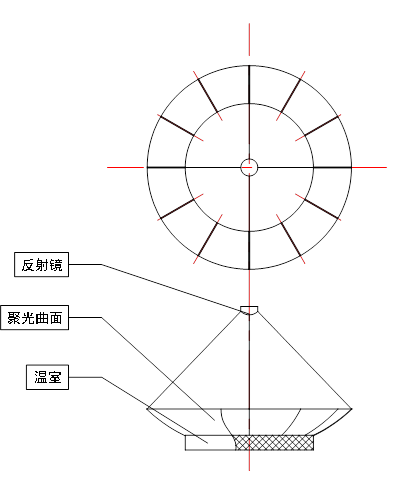
\includegraphics[width=0.5\textwidth]{figure/fanguang-pingmain.png}
  \caption{采光机构平面图}
\end{figure}

根据反射面须使温室接收自身2.311倍的面积的光照,乘上1.1倍安全系数后,得到曲面对地投影的半径为20.73米。并且考虑到反射镜的高度,将凹面镜的曲率半径设为30\si{\meter} 。简图如下:
\begin{figure}[H]
  \centering
  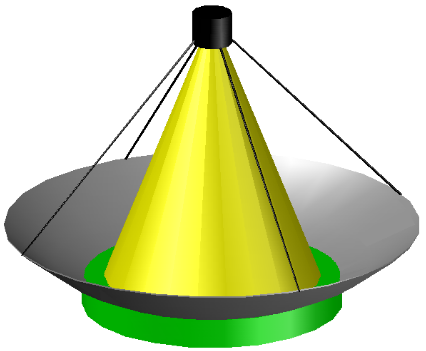
\includegraphics[width=0.4\textwidth]{figure/fanguang-kaideng.png}
  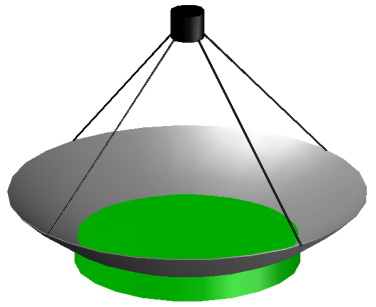
\includegraphics[width=0.4\textwidth]{figure/fanguange-liti.png}
  \caption{采光机构立体图}
\end{figure}

曲面移动机构:  由于使整个结构进行转动使之面向太阳是不理想的,故将凹面镜设计为凹面镜阵列系统,即每块子凹面镜都有其移动机构,使面镜在一个太阳日中光照较强的时候面向太阳,将效率最大化。
镜体自清洁: 用可移动通气杆喷射气体吹除的方式对凹面镜进行自清洁,至于反射镜则由类似于汽车雨刷的方式进行自清洁。移动机构及配气方案从略。
